\chapter{Fine-grained Cross Modal Retrieval}
\label{cha:Method}

In Chapter \ref{cha:scan}, we explained in detail on the structure and principle behind our coarse-grained cross-modal retrieval model. According to the result from running artworks datasets on the baseline model, there are aspects that we can focus on to make improvements. In this chapter, we will present our improved model of fine-grained cross-modal retrieval.

The structure of this chapter is as follows. Section 4.1 gives a brief introduction on our plans for modifying the baseline model into a fragment level. Section 4.2 provides an explanation on the processed artwork datasets and why the pre-processing is necessary for our model. Section 4.3 proposes our improved fine-grained cross modal retrieval model on fragment level instead of focusing on a whole image or sentence. Section 4.4 shows results of our presented model running on our annotated artworks datasets. Section 4.5 points out some existing shortcomings of our methodology and potential fields to be focused on in the future. Section 4.6 concludes this section.


\section{Fragment Retrieval}
In this chapter, we are trying to solve the cross-modal retrieval task in a fine-grained level, which means we shall not limit our retrieval on the image or sentence level but a fragment level. We performed some changes on the baseline model in Chapter \ref{cha:scan}:

\begin{itemize}
    \item Instead of attending between image fragments with each token in sentence captions, here we extract noun phrases from sentence captions to perform mutual attention with image fragments.
    \item During the testing process, we replace the original annotations of artworks but adopt manually handcrafted annotations as ground truth, which shall give us a more accurate experiment result.
\end{itemize}

Next, we present our datasets used in this chapter.

\section{Dataset Preparation}
\label{sec:dataprep}
As we mentioned in Section \ref{cha:intro}, the datasets used in this thesis are from the Rijksmuseum Challenge by Mensink et al. \cite{MensinkICMIR2014}. The raw datasets were downloaded from the webpage dedicated to the Rijksmuseum Challenge. For each artwork, two files were available: a high-resolution \verb|jpeg| image file and an accompanying \verb|xml| file including the metadata.

Python scripts (see Appendix \ref{app:A}) were written to parse the \verb|xml| files. Instead of using the raw captions, here the textual attributes we use are already processed into phrases. The technique here used is from Handler et al. \cite{nounphrase}, it extracts noun phrases from captions in raw \verb|xml| files which potentially helped us improve the accuracy as in most cases noun phrases contains more relevant information of artworks.  

As one single artwork can often have more than one annotation existed in its corresponding \verb|xml| file, it is essential to extract all related annotations out and also combine them into one record for training and testing purpose, which saves computational power and simplifies the model input. 

\subsection{Extract Textual Captions for Each Image}

According to those textual captions and their image labels in \verb|xml| files, we can extract the corresponding image names. This extraction process is done using \verb|egyptian_convert.py| in Appendix \ref{app:A}, the sentence captions for each image will have a corresponding \verb|txt| file created. These obtained \verb|txt| captions will then be processed to extract noun phrases in order to achieve the retrieval in a fragment level; results are saved in \verb|json| format. 

Our training tasks will be based on these noun phrases and extracted image fragments. The following section will demonstrate the architecture of our fine-grained cross-modal retrieval model.

\section{Overall Architecture}

The architecture of the fine-grained cross-modal retrieval model is depicted in Figure \ref{fig:mainarch}. This model takes full artwork images and full sentence captions as input. The full artwork image input is a (224, 224) sized colour high-resolution picture and the full sentence caption comes from the Rijksmuseum dataset \cite{MensinkICMIR2014} which contains several descriptions of artworks.

The model has two pipelines processing image and text input from start, for image input, we first detect salient regions as bottom-up attention \cite{bottomup} to extract features from images using faster R-CNN \cite{fasterrcnn} and ResNet-101 \cite{resnet} (mentioned in Section \ref{sec:fasterrcnn}). These obtained image fragments and their representations will be passed into a fully-connected layer, in order to transform them into a joint embedding space with the same dimension of text (i.e. the dimension of GRU explanation in next paragraph).

For full sentence captions as text input, as we mentioned in Section \ref{sec:dataprep}, we do not process the whole sentence directly but first, extract noun phrases out to achieve a finer-grained level. These noun phrases features will be passed into a bidirectional GRU to map them into the same dimension joint embedding space as image features. 

\begin{figure}[h!]
\centering
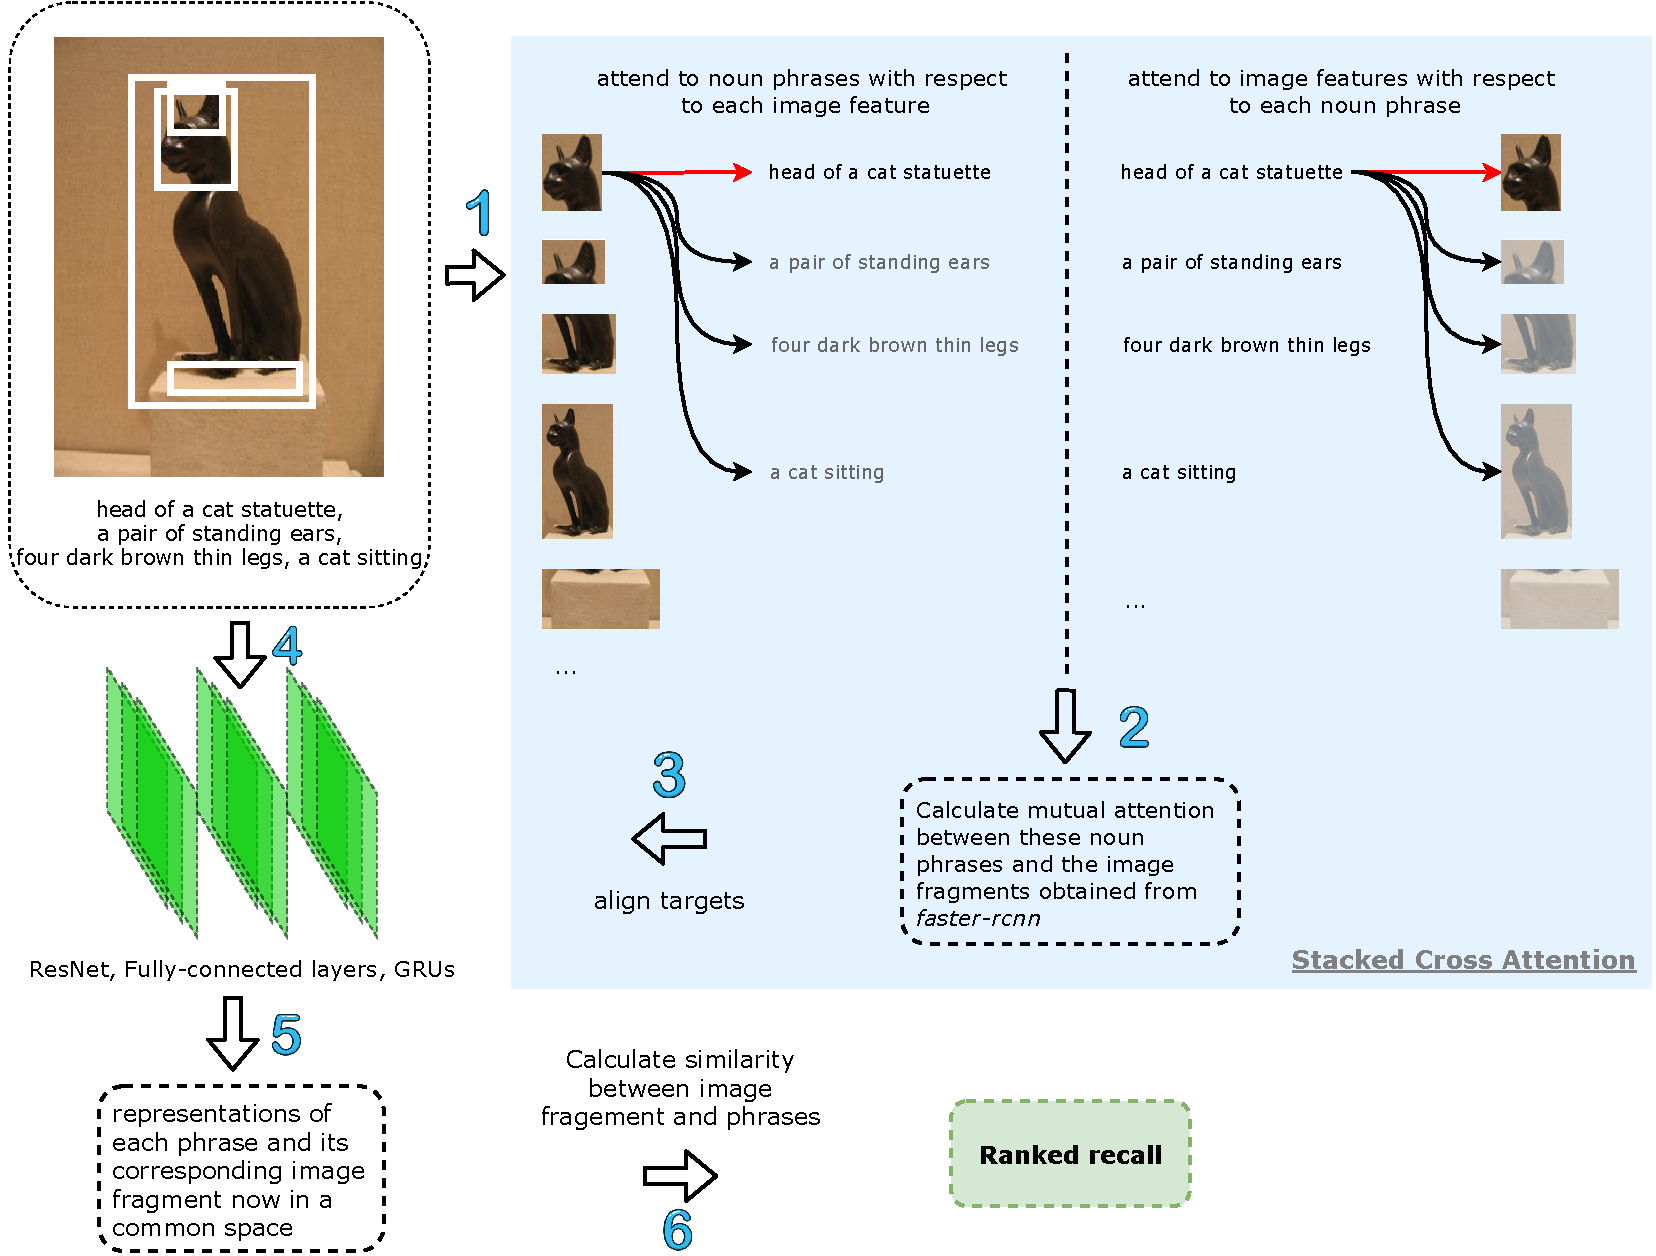
\includegraphics[width=1.0\textwidth]{archi.pdf}
\caption{Fine-grained Cross Modal Retrieval Model Architecture}
\label{fig:mainarch}
\end{figure}

After we learnt image and text representation in a common space, we can use SCAN to attend image to text and attend text to image, in order to get a better alignment in between. After computed mutual attention between image and text, we can start our follow-up part, which is cross-modal retrieval. We can use our learnt common space representation to calculate similarity scores between image and text; meanwhile, calculate ranked precision and recall for testing.

\section{Experiments}

\subsection{Ground Truth}

For this specific task, as we mentioned before, we used our manually annotated ground truth datasets. Each artwork has an updated \verb|xml| file which contains handcrafted image features and textural attributes. Here we show an example of ground truth annotation in Figure \ref{fig:sampledata}.

\begin{figure}[h!]
\centering
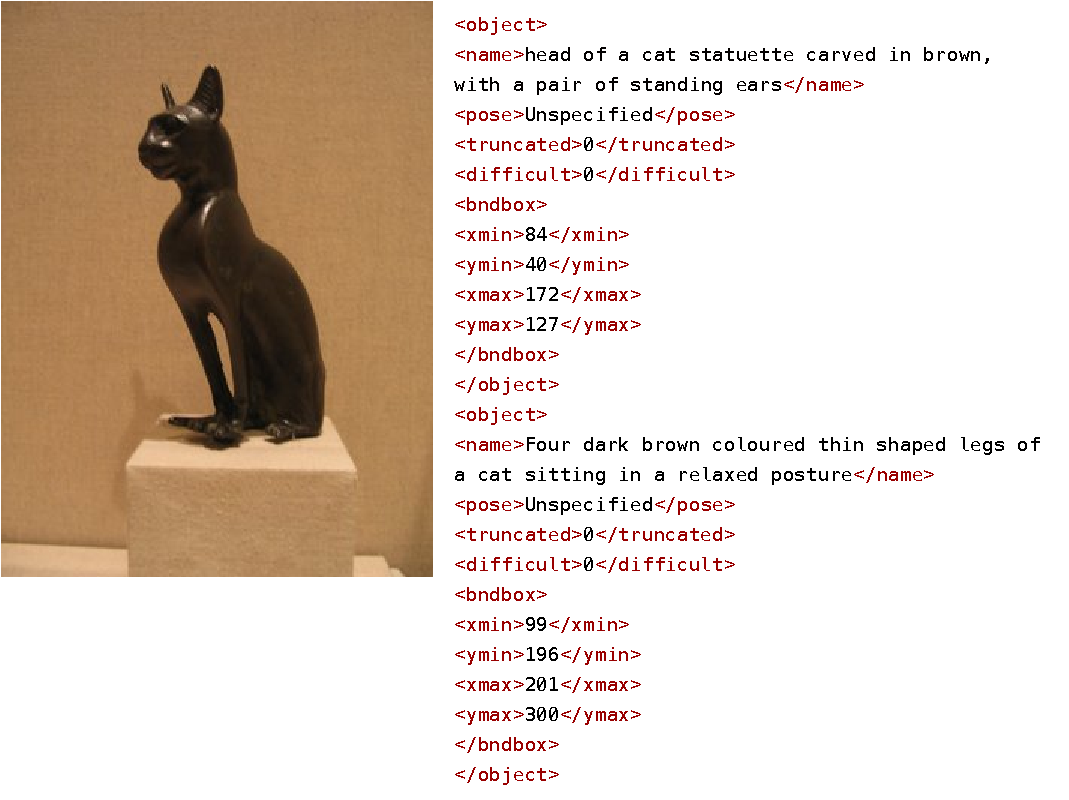
\includegraphics[width=0.8\textwidth]{sampledata.pdf}
\caption{Sample Artwork with Ground Truth Features}
\label{fig:sampledata}
\end{figure}

From Figure \ref{fig:sampledata} we are looking at an Egyptian artwork with a cat sculpture. For all object that exist in the artwork, those are, ``\textit{head of a    cat statuette carved in brown, with a pair of standing ears}'' and ``\textit{four dark brown coloured thin shaped legs of a cat sitting in a relaxed posture}'', each of them will have a corresponding detailed location, pose, and truncated information attached. 

\subsection{Evaluation Metrics}

Recall is one of the most commonly used metrics in the field of information retrieval. Here in this research project, we evaluate the performance of sentence retrieval (image query) and image retrieval (sentence query) by the recall at K (R@K). This is defined as the fraction of queries for which the correct item is retrieved in the closest K points to the query. Details of training and the bottom-up attention implementation are explained in Appendix \ref{app:n}.

\subsection{Results}

\begin{table}[h!]
\centering
\begin{tabular}{lcccccc}
                                                                                                  & \multicolumn{3}{c}{Sentence Retrieval}                                       & \multicolumn{3}{c}{Image Retrieval}                                          \\ \hline
Method                                                                                            & \multicolumn{1}{l}{R@1} & \multicolumn{1}{l}{R@5} & \multicolumn{1}{l}{R@10} & \multicolumn{1}{l}{R@1} & \multicolumn{1}{l}{R@5} & \multicolumn{1}{l}{R@10} \\ \hline
Faster R-CNN, ResNet                                                                              & \multicolumn{6}{c}{Ancient Chinese art alignment dataset}                                                                                                  \\ \hline
SCAN t-i LSE ($\lambda_1$ = 9, $\lambda_2$ = 6)                                                                     & 0.1                     & 0.4                     & 0.8                      & 0.1                     & 0.2                     & 0.6                      \\
SCAN t-i AVG ($\lambda_1$ = 9)                                                                             & 0.1                     & 0.1                     & 0.2                      & 0.1                     & 0.2                     & 0.2                      \\
SCAN i-t LSE ($\lambda_1$ = 4, $\lambda_2$ = 20)                                                                    & 0.1                     & 0.2                     & 0.4                      & 0.1                     & 0.1                     & 0.3                      \\
SCAN i-t AVG ($\lambda_1$ = 4)                                                                             & 0.0                     & 0.2                     & 0.5                      & 0.1                     & 0.2                     & 0.3                      \\ \hline
\begin{tabular}[c]{@{}l@{}}SCAN t-i LSE + i-t AVG\\ (with fragmented image and text)\end{tabular} & \textbf{0.2}            & \textbf{1.2}            & \textbf{2.4}             & \textbf{0.2}            & \textbf{1.0}            & \textbf{2.4}            
\end{tabular}
\caption{Result of Fragmented SCAN on Chinese Artwork Dataset}
\label{table:resultfragmentedCN}
\end{table}

%%%%%%%%

\begin{table}[h!]
\centering
\begin{tabular}{lcccccc}
                                                                                                  & \multicolumn{3}{c}{Sentence Retrieval}                                       & \multicolumn{3}{c}{Image Retrieval}                                          \\ \hline
Method                                                                                            & \multicolumn{1}{l}{R@1} & \multicolumn{1}{l}{R@5} & \multicolumn{1}{l}{R@10} & \multicolumn{1}{l}{R@1} & \multicolumn{1}{l}{R@5} & \multicolumn{1}{l}{R@10} \\ \hline
Faster R-CNN, ResNet                                                                              & \multicolumn{6}{c}{Ancient Egyptian art alignment dataset}                                                                                                  \\ \hline
SCAN t-i LSE ($\lambda_1$ = 9, $\lambda_2$ = 6)                                                                     & 0.1                     & 0.4                     & 0.8                      & 0.1                     & 0.2                     & 0.6                      \\
SCAN t-i AVG ($\lambda_1$ = 9)                                                                             & 0.1                     & 0.1                     & 0.2                      & 0.1                     & 0.2                     & 0.2                      \\
SCAN i-t LSE ($\lambda_1$ = 4, $\lambda_2$ = 20)                                                                    & 0.1                     & 0.2                     & 0.4                      & 0.1                     & 0.1                     & 0.3                      \\
SCAN i-t AVG ($\lambda_1$ = 4)                                                                             & 0.0                     & 0.2                     & 0.5                      & 0.1                     & 0.2                     & 0.3                      \\ \hline
\begin{tabular}[c]{@{}l@{}}SCAN t-i LSE + i-t AVG\\ (with fragmented image and text)\end{tabular} & \textbf{0.7}            & \textbf{3.7}            & \textbf{8.1}             & \textbf{0.7}            & \textbf{3.7}            & \textbf{9.6}            
\end{tabular}
\caption{Result of Fragmented SCAN on Egyptian Artwork Dataset}
\label{table:resultfragmentedEG}
\end{table}

\section{Future Works}
Besides focusing on the fragment level image/sentence retrieval, it would also be beneficial to consider adopting a new image representation. 

Recently, some works \cite{TranslatingArtworks,parttowhole,Art2Real} have proposed new frameworks for artwork feature extraction and made prominent progress in the field. 


\section{Conclusion}


%%% Local Variables: 
%%% mode: latex
%%% TeX-master: "thesis"
%%% End: 
